% Asset ID: A21FunctionsAndGraphsTIKZ-006
% Unit: A21: A2 1 Pure Mathematics
% Topic code: A21-AF
% Related LO IDs: A21-AF-LO005
% Related lesson section: Graphing an Inverse Function
% Source: Chapter 2 Functions and Graphs inverse function section
% Purpose: Show that inverse-function graphs are reflections in y = x.

\documentclass[tikz,border=8pt]{standalone}
\usepackage{amsmath}
\usetikzlibrary{arrows.meta}
\begin{document}
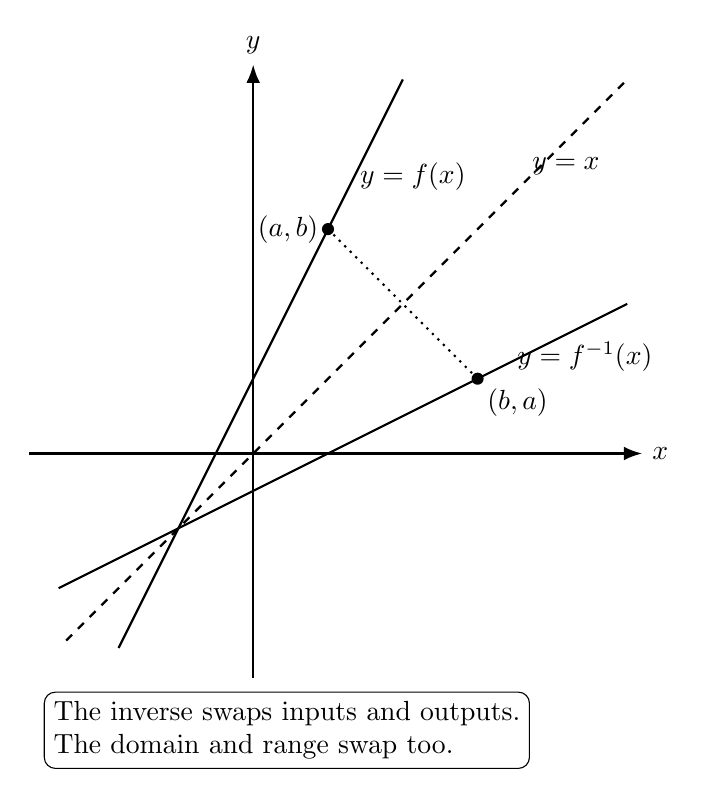
\begin{tikzpicture}[scale=0.95, >=Latex]
\draw[->, thick] (-3,0) -- (5.2,0) node[right] {$x$};
\draw[->, thick] (0,-3) -- (0,5.2) node[above] {$y$};
\draw[dashed, thick] (-2.5,-2.5) -- (5,5);\node[above right] at (3.6,3.6) {$y=x$};
\draw[thick] (-1.8,-2.6) -- (2,5);\node[right] at (1.3,3.7) {$y=f(x)$};
\draw[thick] (-2.6,-1.8) -- (5,2);\node[right] at (3.4,1.3) {$y=f^{-1}(x)$};
\fill (1,3) circle (2.3pt);\fill (3,1) circle (2.3pt);\draw[dotted, thick] (1,3) -- (3,1);
\node[left] at (1,3) {$(a,b)$};\node[below right] at (3,1) {$(b,a)$};
\node[align=left, draw, rounded corners, anchor=west] at (-2.8,-3.7) {The inverse swaps inputs and outputs.\\The domain and range swap too.};
\end{tikzpicture}
\end{document}
